%----------------------------------------------------------------------------
\chapter{\projectlifecycle}
%----------------------------------------------------------------------------

A projektmenedzsment egyik legfontosabb alapelve, hogy minden projektnek megvan a maga életciklusa, 
amely jól elkülöníthető fázisokra bontható. 
Ezek a fázisok nemcsak logikai, hanem szervezeti és irányítási szempontból is meghatározóak, 
hiszen lehetővé teszik a projekt strukturált tervezését, nyomon követését és értékelését. 
A hazai szakirodalom egyaránt öt alapvető fázist különít el \cite{Szalay2018,Hajdu2014}:

\begin{enumerate}
    \item \textbf{Projektindítás (Initiation)} a projekt céljainak, indokoltságának és alapvető paramétereinek meghatározása.
    \item \textbf{Tervezés (Planning)} az ütemezés, erőforrások, kockázatok és feladatok részletes kidolgozása.
    \item \textbf{Megvalósítás (Execution)} a tényleges fejlesztési és kivitelezési folyamatok végrehajtása.
    \item \textbf{Ellenőrzés és irányítás (Monitoring \& Controlling)} a projekt előrehaladásának, költségeinek és minőségének nyomon követése.
    \item \textbf{Lezárás (Closure)} a projekt hivatalos befejezése, átadás és értékelés.
\end{enumerate}

%----------------------------------------------------------------------------
\begin{figure}[H]
    \centering
    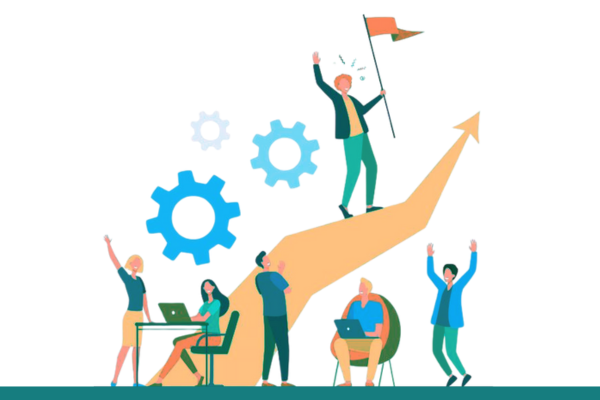
\includegraphics[width=75mm, keepaspectratio]{figures/project_creative.png}
    \caption{Projekt kreatív vizualizáció}
    \label{fig:project_creative}
\end{figure}
%----------------------------------------------------------------------------

A projektciklus fázisai egymásra épülnek, ugyanakkor gyakran átfedésben is lehetnek: 
az ellenőrzési és irányítási folyamat például a megvalósítás teljes ideje alatt folyamatosan zajlik.  
A modern megközelítések különösen az iteratív és ismétlődő fejlesztési modellek nem mindig lineáris struktúrát követnek, 
hanem sprint vagy iteráció formájában valósítják meg a fejlesztést.  

Ennek ellenére a klasszikus projektciklus továbbra is nélkülözhetetlen a stratégiai és vállalati projektekben, 
mivel jól követhető keretet biztosít az egész folyamat számára.  

A \textbf{TeDeRMS} fejlesztésénél egy klasszikus, ötfázisú modell szolgált alapul, 
melyet a projekt egyedi körülményeihez önálló fejlesztés, korlátozott erőforrások, vállalati integráció igazítottam.  
Az alábbiakban részletesen bemutatom, hogyan valósult meg a projekt életciklusa a gyakorlatban.


%----------------------------------------------------------------------------
\section{Projektindítás (Initiation)}
%----------------------------------------------------------------------------

A projektindítás során a következő lépések történtek:
\begin{itemize}
    \item \textbf{Igényfelmérés:} a vállalat bérléskezelési folyamatait elemeztem, hogy pontosan feltérképezzem a fejlesztendő rendszer funkcióit és a problémás területeket.
    \item \textbf{Célok meghatározása:} világos, mérhető célkitűzéseket rögzítettem, például az adminisztrációs idő csökkentését, a hibák minimalizálását és az automatizált riportok bevezetését.
    \item \textbf{Erőforrás-tervezés előkészítése:} meghatároztam a projekthez szükséges technológiai és időbeli erőforrásokat. 
    Mivel a fejlesztést önállóan végeztem, kiemelten fontos volt a prioritások és a munkaidő hatékony beosztása.
\end{itemize}

Ez a fázis biztosította, hogy a projekt kiindulópontja egyértelmű legyen, és a fejlesztés a vállalat igényeinek megfelelően induljon el.
Amennyiben a projektindítás nem lett volna alapos, a későbbi fázisokban jelentős problémák merülhettek volna fel, 
például félreértett követelmények esetében a fejlesztés nem a kívánt irányba haladt volna ezzel erőforrásokat és időt pazarolva.

%----------------------------------------------------------------------------
\section{Tervezés (Planning)}
%----------------------------------------------------------------------------

A tervezési fázisban a projekt sikerének záloga a részletes ütemezés és a kockázatok előrejelzése volt:
\begin{itemize}
    \item \textbf{Ütemterv készítése:} a projekt főbb mérföldköveit és feladatait időrendi sorrendbe állítottam, így követhetővé vált a fejlesztés előrehaladása.
    \item \textbf{Erőforrás-tervezés:} részletesen meghatároztam az idő- és technológiai erőforrásokat, valamint a napi munkabeosztást, hogy az önálló fejlesztés gördülékeny legyen.
    \item \textbf{Kockázatelemzés:} azonosítottam a legfontosabb kockázatokat (pl. technikai hibák, adatvesztés, hibás üzleti logika), és kidolgoztam a megelőző és elhárító intézkedéseket.
\end{itemize}

A tervezés során alkalmazott módszerek: feladatlista, ütemezett mérföldkövek, kockázatmátrix és rendszeres önellenőrzés.

%----------------------------------------------------------------------------
\section{Megvalósítás (Execution)}
%----------------------------------------------------------------------------

A megvalósítás során a projekt tényleges fejlesztési munkája zajlott:
\begin{itemize}
    \item \textbf{Fejlesztési folyamatok:} moduláris felépítésben, backend és frontend párhuzamos fejlesztése, verziókövetés GitHub-on.
    \item \textbf{Tesztelés:} folyamatos unit és funkcionális tesztek, hogy a rendszer stabil és hibamentes legyen.
    \item \textbf{Dokumentáció:} a kód és a rendszer működésének részletes dokumentálása, hogy a későbbi karbantartás és bővítés egyszerű legyen.
\end{itemize}

Ez a fázis biztosította, hogy a rendszer minden funkciója a terv szerint valósuljon meg, és a vállalat igényei teljesüljenek.

%----------------------------------------------------------------------------
\section{Ellenőrzés és irányítás (Monitoring és Controlling)}
%----------------------------------------------------------------------------

A projekt előrehaladásának nyomon követése kritikus volt a siker szempontjából:
\begin{itemize}
    \item \textbf{Haladás nyomon követése:} a mérföldkövek teljesülésének ellenőrzése, eltérések azonosítása és korrekciója.
    \item \textbf{Kockázatok kezelése:} a kockázatmátrix folyamatos frissítése, a problémák gyors azonosítása és megoldása.
    \item \textbf{Minőségellenőrzés:} a rendszer funkcionalitásának és stabilitásának folyamatos ellenőrzése a hibák minimalizálása érdekében.
\end{itemize}

Ez a fázis biztosította, hogy a projekt ne csússzon ki a tervezett keretek közül, és minden mérföldkő a kívánt minőségben valósuljon meg.

%----------------------------------------------------------------------------
\section{Projekt lezárás (Closure)}
%----------------------------------------------------------------------------

A projekt lezárásakor a következő tevékenységek történtek:
\begin{itemize}
    \item \textbf{Rendszer átadása:} a \textbf{TeDeRMS} teljes körű telepítése a vállalat környezetében.
    \item \textbf{Dokumentáció:} részletes használati útmutatók és adminisztrátori kézikönyvek készítése.
    \item \textbf{Oktatás:} a kulcsfelhasználók képzése a rendszer hatékony használatára.
    \item \textbf{Tanulságok összegzése:} a projekt során szerzett tapasztalatok dokumentálása, javaslatok a jövőbeli bővítésekhez.
\end{itemize}

Ez a fázis biztosította, hogy a rendszer hosszú távon stabilan és hatékonyan működjön, 
miközben a projektmenedzsment folyamatok tanulságai később is felhasználhatók.
